\documentclass[border=2pt]{standalone}
\usepackage{tikz,amsmath}
\begin{document}
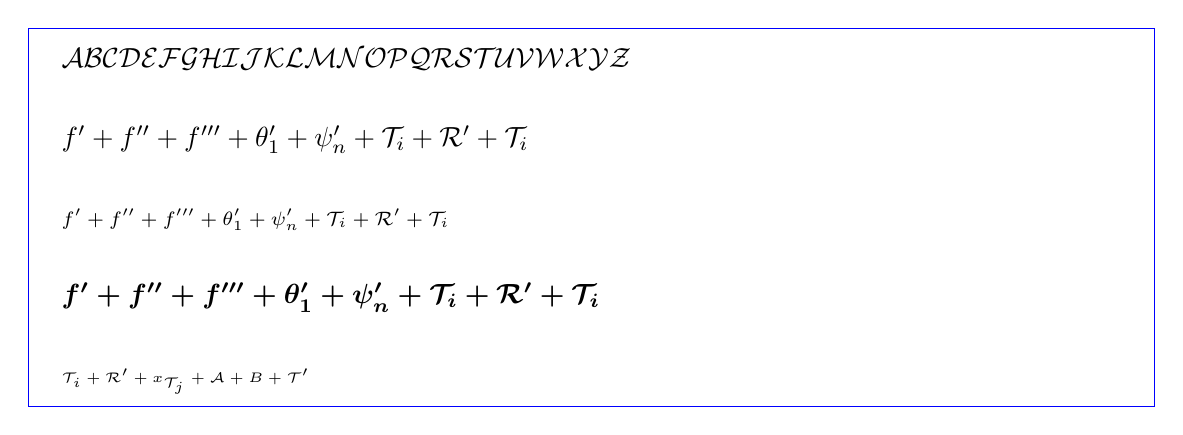
\begin{tikzpicture}
  \draw[blue] (-.3,-4.3) rectangle (14,.5);
  \node[anchor=base west] at (0,0)
    {$\mathcal{ABCDEFGHIJKLMNOPQRSTUVWXYZ}$};
  \node[anchor=base west] at (0,-1)
    {$f'+f''+f''' + \theta_1' + \psi_n' + \mathcal{T}_i + \mathcal{R}' + {\mathcal{T}}_i$};
  \node[anchor=base west,font=\scriptsize] at (0,-2)
    {$f'+f''+f''' + \theta_1' + \psi_n' + \mathcal{T}_i + \mathcal{R}' + {\mathcal{T}}_i$};
  \node[anchor=base west,font=\boldmath] at (0,-3)
    {$f'+f''+f''' + \theta_1' + \psi_n' + \mathcal{T}_i + \mathcal{R}' + {\mathcal{T}}_i$};
  \node[anchor=base west,font=\tiny] at (0,-4)
    {$\mathcal{T}_i + \mathcal{R}' + x_{\mathcal{T}_{j}} + \mathcal{A}+B+\mathcal{T}'$};
\end{tikzpicture}
\end{document}
